\documentclass{article}
\usepackage{graphicx}
\usepackage{siunitx}
\graphicspath{ {images/} }
\title{First Pully Problem}
\author{Grant Curell}
\begin{document}
\maketitle{}
\section{Problem}
For example, take a look at Figure 5-9, where you’ve started your own grocery store and bought a wire rated at 15 newtons to hang the sign with. The sign weighs only 8.0 newtons, so hanging it should be no problem, right? Obviously, you can tell from my phrasing that you have a problem here. Coolly, you get out your calculator to figure out what force the wire, F1 in the diagram, has to exert on the sign to support it.

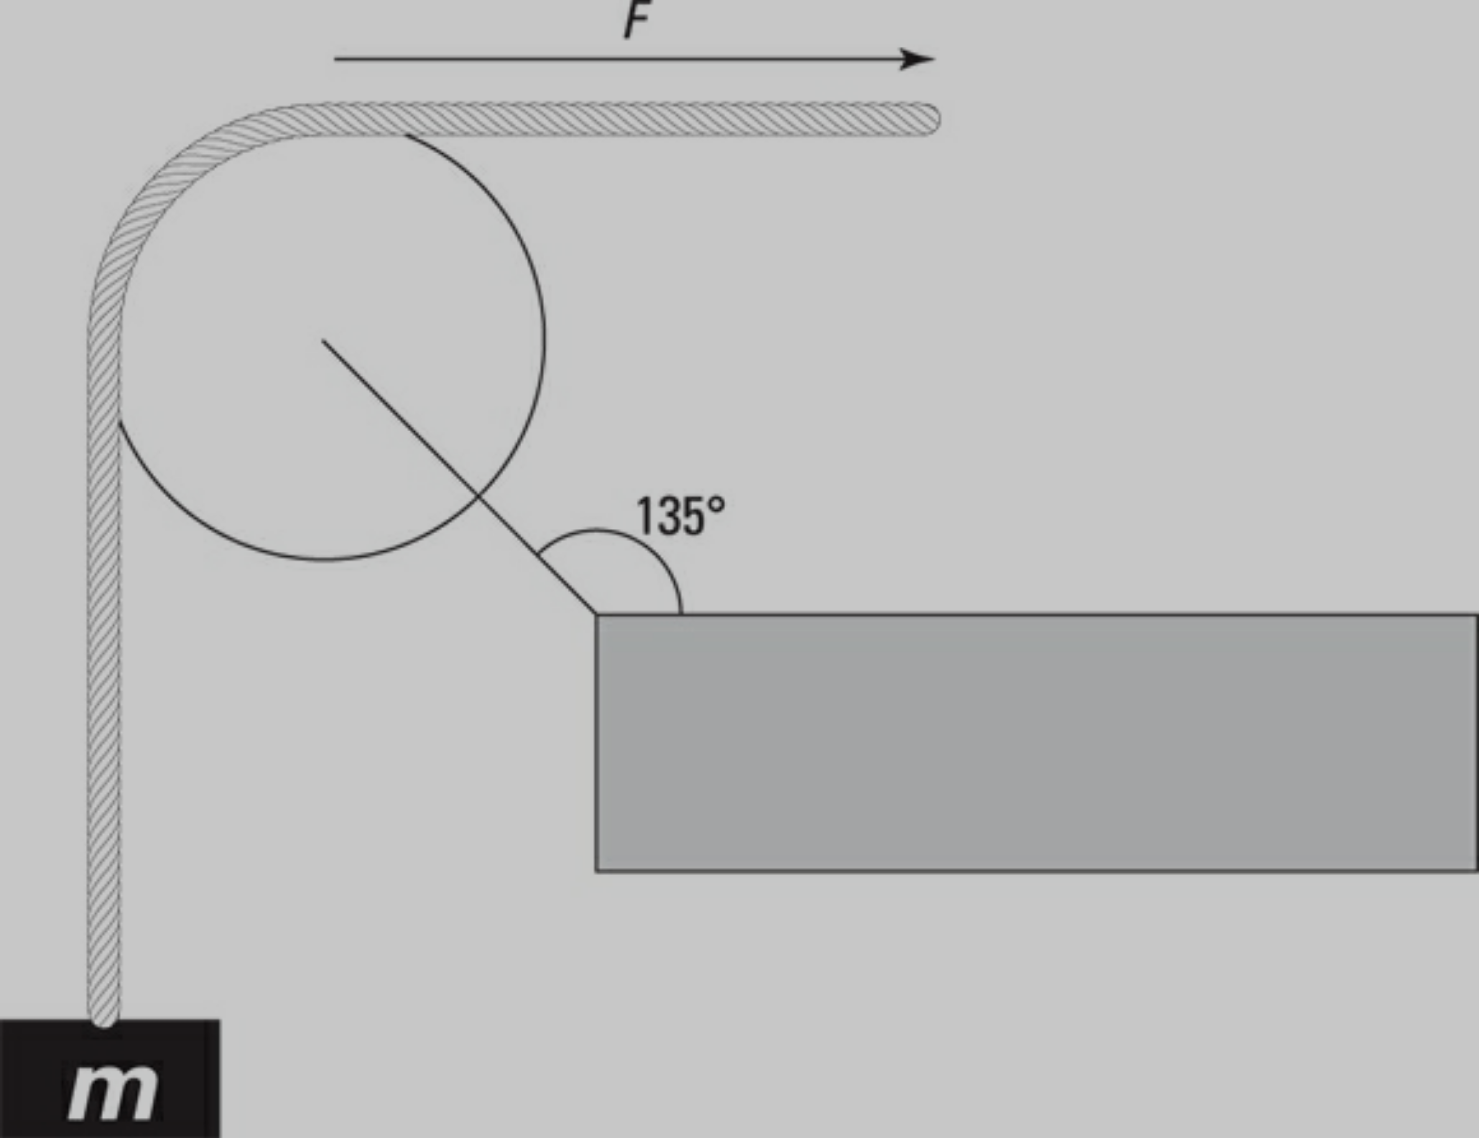
\includegraphics[width=\columnwidth]{image}
\\\\
Holzner, Steven. Physics I For Dummies (For Dummies (Math \& Science)) (p. 97). Wiley. Kindle Edition.
\\\\
\section{Solution}
\[ \sum F_y=F_{mass} \]
\[ \sum F_x=F_{manmeat pulling} \]
\[ \sum F_x=9.8m \]
\[ \sum F_y=-9.8m \]
Puesto que la acceleración del sistema es 0, sigue que las fuerzas tendrían
que igualar zero.
\[ \sum F_{support}=(-9.8m,9.8m) \]
\[ \sum F_{support}=\sqrt{(-9.8m)^2+(9.8m)^2} \]
The angle would be the same as the support so 135 degrees.
\end{document}
